\section{Desarrollo}
	\subsection {Tecnologías y Software empleados}
	\begin{itemize}
		\item IntelliJ IDEA 2023.1.2 (Ultimate Editon)
		\item Java correto-17 versión 17.0.17)
		\item Git versión 2.34.1
		\item MySQL Workbench 8 versión 8.0.32
		\item Mysql Ver 8.0.33-0ubuntu0.22.04.2
		\item Spring Boot 3.0.1
		\item Ubuntu 22.04 LTS
		\item Postman v10.15.1
	\end{itemize}
	\subsection{Procedimiento}
	Desde un requerimiento general se debe realizar un análisis a profundidad sobre las necesidades, dicho análisis debe ser genérico; es decir debe valer para cualquier aplicación que requiera de esa funcionalidad.\\
	
	Una vez teniendo el análisis se revisa la documentación de Spring Boot sobre la implementación de los microservicios, con esto podemos transportar el análisis realizado en papel a código de programación, en este caso utilizamos Java como lenguaje de programación principal apoyándonos de un framework que facilita la implementación de funcionalidades que son demandantes de tiempo al estar desarrollando como lo es la conexión a base de datos, facilidad en integrar dependencias, facilidad de visualizar el desarrollo en el navegador integrando un contenedor de aplicaciones web para ser desplegado.
	
	\subsubsection{Patrón MVC}
	Utilizamos el patrón de desarrollo MVC para logar la estructura de carpetas ordenadas sin mezclar la lógica de negocio con la funcionalidad a implementar. El patrón de desarrollo MVC se compone de esta estructura:
	\begin{itemize}
		\item Modelos: Representan los datos y la lógica de negocio de la aplicación, con ellas gestionamos las entidades de las bases de datos, validaciones a nivel de tipo de datos y limitantes de aceptación.
		En estos componentes es donde se establece la cardinalidad de las entidades a utilizar.
		\item Vista: Es la interfaz de usuario de la aplicación, se encarga de la representación visual de los datos y la interacción con el usuario, en este caso omitimos esta parte en microservicios ya que estos solo devuelven colecciones de tipo Json o xml según sean las necesidades de la aplicación a escalar.
		\item Controlador: Actuá como intermediario entre el modelo y la vista, además su parte principal es controlar el flujo de la aplicación, coordinando las diferentes acciones y actualizaciones internas del sistema.
	\end{itemize}
	\begin{minipage}{0.3\textwidth}
		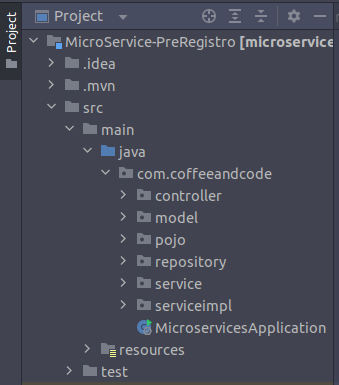
\includegraphics[width=\linewidth]{img/mvc.png}
	\end{minipage}
	\hfill
	\begin{minipage}{0.7\textwidth}
		Se decide utilizar este patrón de desarrollo, debido a que permite la modularidad y flexibilidad en el desarrollo de nuestro microservicio, cada componente tiene una responsabilidad especifica y se puede modificar o remplazar de manera independiente, la ejemplificación del patrón MVC la podemos observar en la siguiente imagen.
	\end{minipage}
	
	\subsubsection{Servicios, interfaces de repositorios, implementación de interfaces.}
	Una de las facilidades que permite Spring Boot es la inyección de dependencias, con estas se hace referencia a los servicios e interfaces de repositorios, en otros componentes, esto similar al funcionamiento de los controladores.\\
	Se utilizan para dividir las responsabilidades y facilitar la prueba y mantenimiento del código, se podría decir que también son pieza importante donde se permite la modularidad, escalabilidad y flexibilidad del sistema.
	\begin{itemize}
		\item Servicios: Aquí se implementa la lógica de negocio de una aplicación, representan la capa intermedia entre los controladores y los repositorios, con ellas se busca proporcionar funcionalidad especifica y operaciones más complejas.
		\item Interfaces de repositorios: Definen métodos para interactuar con la capa de almacenamiento de datos(bases de datos, o servicios web). Permiten la abstracción de la lógica de acceso a datos y proporcionan una forma estandarizada para las operaciones CRUD(Crear, Leer, Actualizar, Eliminar) sobre los objetos persistentes. 
		\item Implementación de interfaces: Contienen la creación de clases que implementan las interfaces definidas, dichas clases contienen la lógica concreta para llevar a cabo las operaciones definidas en las interfaces, es decir aquí es en donde se desarrolla el método completo.
	\end{itemize}
	
	
	
	\subsubsection{Desarrollo de microservicios}
	Iniciamos con el proceso de desarrollo de microservicios, primero definimos que tipo de datos aceptará y entregará nuestro microservicio, para este caso especifico se decide que será en Json.\\
	
	Utilizando MVC definimos las entidades de nuestra base de datos en el apartado \textbf{model}, en este se establece la cardinalidad que hemos definido en nuestro diagrama entidad relación que diseñamos durante el análisis de requerimientos, es aquí donde definimos los atributos que contendrá la tabla, ademas del nombre de la misma todo con notaciones que pertenecen a dependencias utilizadas para \textbf{maven} apoyados del framework \textbf{Spring Boot.}

	
	
	
	
	
	Describe tus diagramas de clase utilizado en caso de  haber todos elementos empleados.
	
\subsection{Resultados}
Aquí describir los resultados obtenidos evidencia del programa funcionando y describir las funcionalidades puedes incluir imágenes.